% !TeX spellcheck = <none>
% !TeX encoding = UTF-8
% !TeX root = main.tex

\chapter{LiDAR工程数据获取}%% Chapter05 LiDAR工程数据获取

\paragraph{LiDAR工程步骤}如图\ref{fig:LiDAR工程步骤}所示。
\begin{figure}[h]
	\centering
	\begin{tikzpicture}[
		terminal/.style = {
			rectangle,minimum size=6mm,rounded corners=3mm,
			very thick,draw=black!50,
			top color=white,bottom color=black!20,
			font=\bfseries
		},
		>=stealth',thick,black!50,text=black,
		graphs/every graph/.style={edges=rounded corners}]
		\matrix[row sep=1mm,column sep=3em] {
			\node    [terminal] (start)		{项目启动}; &
			\node    [terminal]	(get)		{数据获取}; &
			\node    [terminal]	(process)	{数据处理}; &
			\node    [terminal]	(assest)	{精度评定}; &
			\node    [terminal]	(handin)	{提交成果}; \\
		};
		\graph[use existing nodes]{
			start -> get -> process -> assest -> handin;
		};
	\end{tikzpicture}
	\caption{LiDAR工程步骤}
	\label{fig:LiDAR工程步骤}
\end{figure}

\paragraph{LiDAR数据获取综述}
既繁琐又细致的工作,牵扯到许许多多的因
素,需要很多单位和人员的支持和配合。
包含了从飞行准备到航线设计,从飞行操作到
数据整理,从设备运输到存储维护等方方面面
与航测外业相关的作业环节。

\paragraph{三个阶段八个方面}如图\ref{fig:LiDAR数据获取的三个阶段八个方面}所示。
\begin{figure}[htbp]
	\centering
	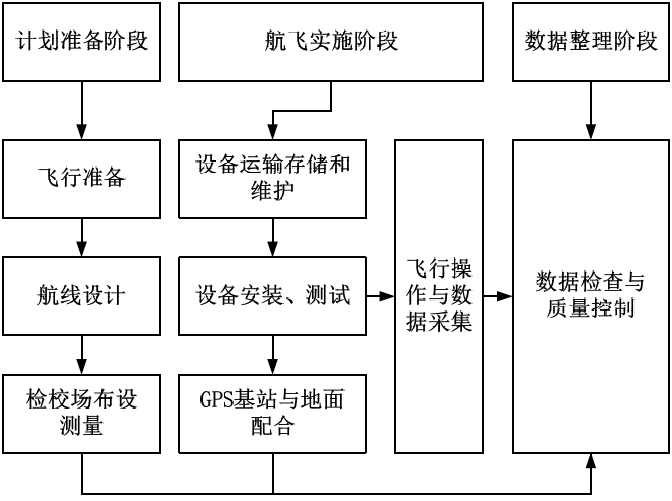
\includegraphics[width=0.7\linewidth]{figure/Chapter5/LiDAR数据获取的三个阶段八个方面}
	\caption{LiDAR数据获取的三个阶段八个方面}
	\label{fig:LiDAR数据获取的三个阶段八个方面}
\end{figure}

\section{LiDAR数据获取流程}
\subsection{计划准备阶段}

\paragraph{飞行准备}
\begin{enumerate}
	\item \textbf{掌握测区情况}。首先应该熟悉实地测区的地形特点和地貌特征。根据不同的地形条件选择和设计不同的飞行航线。
	\item \textbf{选择LiDAR型号}。国内主要有ALS、ALTM、LiteMapper、 TOPOSYS等产品,每个产品由于性能和参数不同,因此选择不同的设备对于航摄设计来说也是不同的。
	\item \textbf{选择飞行平台}。不同的飞机性能会对雷达系统的参数设置有不同程度的影响。主要有两个方面,一是飞行速度,二是飞行高度。
		\begin{itemize}
			\item 飞行速度主要影响雷达的扫描频率的设置。
			\item 行高度主要影响脉冲频率的设置,进而影响点密度和精度。
		\end{itemize}
	\item \textbf{申请航飞权、协调航空飞行}。流程如图\ref{fig:申请航飞权与协调航空飞行}所示。
		\begin{itemize}
			\item 飞行任务审批。
			\item 机场协调。
			\item 飞行协调。
		\end{itemize}
		\begin{figure}[htbp]
			\centering
			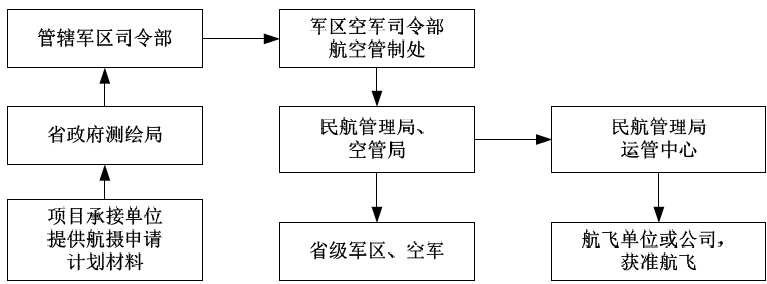
\includegraphics[width=0.7\linewidth]{figure/Chapter5/申请航飞权与协调航空飞行}
			\caption{申请航飞权与协调航空飞行}
			\label{fig:申请航飞权与协调航空飞行}
		\end{figure}
	\item \textbf{制定项目任务书}。在承接航飞任务时,用户单位一般会提交 “项目任务书” ,一般由甲方提出要求,双方技术人员共同拟定。
		\begin{itemize}
			\item 飞行高度
			\item 飞机型号
			\item 航摄分区
			\item 成果坐标系
			\item 野外控制点量测
		\end{itemize}
	\item \textbf{评估飞行效率}。根据测区远近、飞行高度、空域申请情况来编排航飞航线顺序。
\end{enumerate}

\paragraph{航线设计}
\begin{enumerate}
	\item \textbf{步骤}:
		\begin{itemize}
			\item 建立航带设计工程
			\item 设置平面坐标系和高程坐标系
			\item 加载DTM数据
			\item 导入设计线位
			\item 航带设计
			\item 重复以上步骤,完成所有航段的航线设计
		\end{itemize}
		航线设计流程如图\ref{fig:航线设计流程}所示。
		\begin{figure}[htbp]
			\centering
			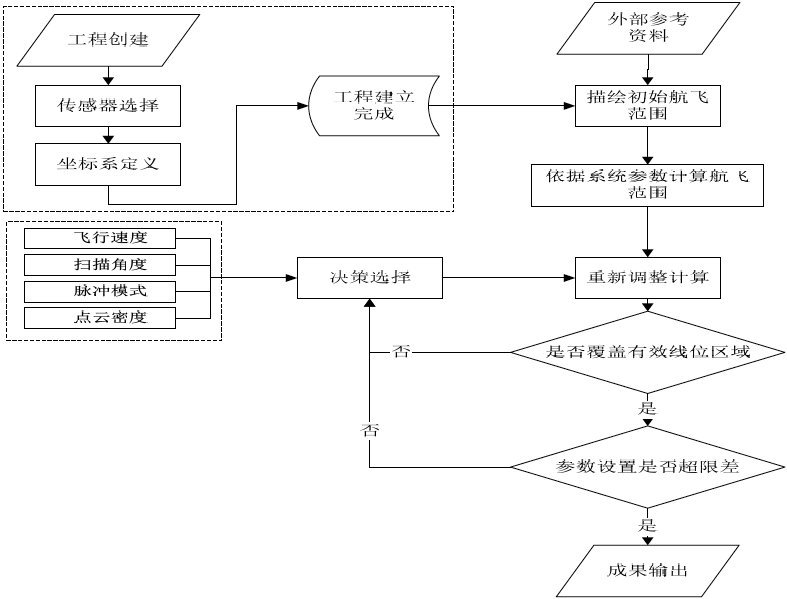
\includegraphics[width=0.7\linewidth]{figure/Chapter5/航线设计流程}
			\caption{航线设计流程}
			\label{fig:航线设计流程}
		\end{figure}
	\item \textbf{单脉冲和多脉冲}:同等点间距的设计要求下,多脉冲的航飞效率大约为单脉冲的3倍!多脉冲的优势随着地形起伏变化的上升而越加明显。
	\item \textbf{配备数码相机的航线设计}:注意
		\begin{itemize}
			\item 重叠度匹配
			\item 数码相机航向重叠度设置和摄影基线检查
		\end{itemize}
	\item \textbf{最终航线检查与地面模拟飞行}:为了确保飞行计划的正确性。检查方法主要有三种:
		\begin{itemize}
			\item 将飞行计划导出为KML格式,加载到Google Earth当中进行浏览。
			\item 将飞行计划导出到FCMS飞行管理控制软件中进行检查。
			\item 地面模拟飞行。
		\end{itemize}
	\item \textbf{提交航飞设计数据}:完成航线设计之后,需要提交以下材料:
		\begin{itemize}
			\item 飞行记录表
			\item 领航数据表
			\item 飞行文件
			\item 飞行示意图文件
			\item KML文件
		\end{itemize}
\end{enumerate}

\paragraph{检校场的布设、量测}
\begin{enumerate}
	\item \textbf{必要性}:LiDAR设备属于精密仪器,数据采集时要求部件之间有严格的相对位置关系。
		但实际工作中,系统安装时不能完全保证它们相互平行,这些偏差会在设备运输中、设备安装时或者随着时间改变。
	\item \textbf{激光检校场选择及航线设计}:IMU和激光扫描仪的坐标系并不严格平行引起的误差;每次航飞过程中,roll、pitch、heading等会发生变化。
		\begin{itemize}
			\item \textbf{激光检校场布设方案}
				\begin{itemize}
					\item \textit{校准控制场}:校准LiDAR的相对和绝对高程。
					\item \textit{校准建筑物}:校准侧滚和俯仰姿态。
					\item 尽量远离水面(如湖、江)等低反射率的地区。
				\end{itemize}
			\item \textbf{激光检校控制点布设方案}
				\begin{itemize}
					\item 直线控制点:直线大路,2km,每隔5m一个, 高程精度<5cm;
					\item 零散控制点:中心区域均匀10-15点,高程精度 <2cm;
					\item 所有控制点都布设在路面上,且地物材料均匀。
					\item 控制点数据的坐标系为WGS84。
				\end{itemize}
			\item \textbf{激光航线设计方案}:如图\ref{fig:激光检校场布设案例}所示。
				\begin{itemize}
					\item 高航高:通过尖顶房屋正上方过房屋中点,垂直道路及房屋的顶角方向往返飞行各一次(EF、FE);平行于该方向飞行一次(CD);沿道路方向同向飞行一次(AB)。
					\item 低航高:十字飞行(EF,BA)。
				\end{itemize}
				\begin{figure}[htbp]
					\centering
					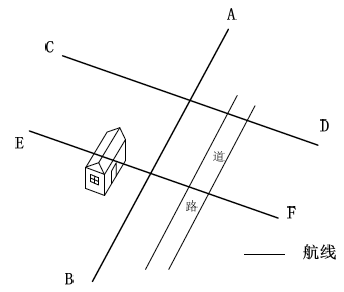
\includegraphics[width=0.4\linewidth]{figure/Chapter5/激光检校场布设案例}
					\caption{激光检校场布设案例}
					\label{fig:激光检校场布设案例}
				\end{figure}
		\end{itemize}
	\item \textbf{相机检校场选择及航线设计}:相机在安装过程中也会存在和IMU的视准轴不严格一致的情况,这就需要在飞行前或飞行后进行视准轴检校 。
		\begin{itemize}
			\item \textbf{相机检校场布设方案}:从不同方向航线的数据中获取尽可能多的同名地物点,且每一个同名地物点所涉及的航片数量尽可能的多,通过对大量同名点的平差计算,求出相机视准轴与IMU之间的偏差。
				检校场可选择在地物比较丰富的城市地区,覆盖范围一般为6.0 km×4.5 km。城市区域可供选择的特征点比较多,适于后续进行空三计算并寻找足够的连接点,得到较好的检校结果。
			\item \textbf{相机航线设计方案}:相机的焦距不同,检校飞行的航高也不同,一般飞1个高度,采用“十”字对飞,四条航线。如图\ref{fig:相机航线设计方案}所示。
				\begin{figure}[htbp]
					\centering
					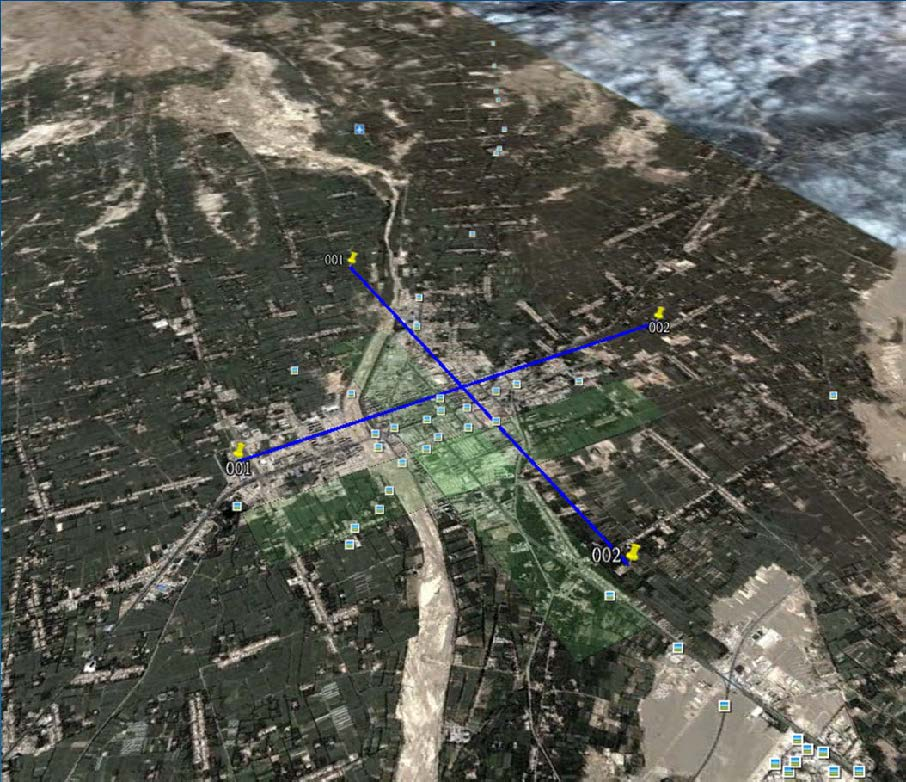
\includegraphics[width=0.7\linewidth]{figure/Chapter5/相机航线设计方案}
					\caption{相机航线设计方案}
					\label{fig:相机航线设计方案}
				\end{figure}
			\item \textbf{相机检校控制点布设方案}:
				\begin{itemize}
					\item 测区范围内均匀布设20个控制点,在重叠中心区布设5$ \sim $10个控制点,在航线四个边缘区域总共布设5$ \sim $10个控制点,精度<5 cm。
					\item 控制点选取地物特征点上。
					\item 控制点数据的坐标系为WGS84。
				\end{itemize}
		\end{itemize}
\end{enumerate}

\paragraph{设备安装与测试}
\begin{enumerate}
	\item 开箱验货与货物清点。
	\item 设备安装步骤
		\begin{itemize}
			\item 飞机改造(GPS天线、底舱过渡板、底舱开孔直径与底舱厚度)。
			\item GPS偏心分量测量。如图所示。
				\begin{figure}[htbp]
					\centering
					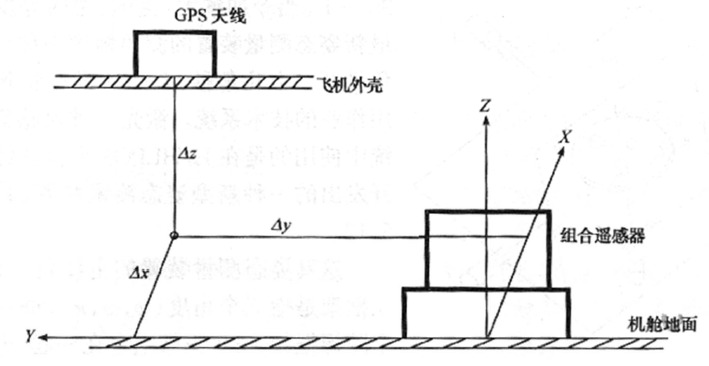
\includegraphics[width=0.7\linewidth]{figure/Chapter5/GPS偏心分量测量}
					\caption{GPS偏心分量测量}
					\label{fig:GPS偏心分量测量}
				\end{figure}
			\item 设备地面通电测试、记录。
			\item 温度处理。
			\item 数据质量检查与设备状态评估。
		\end{itemize}
\end{enumerate}

\subsection{航飞实施阶段}

\paragraph{基站架设与地面配合}地面配合分为
\textit{检校场地面配合}\footnote{检校场地面配合是针对检校场开展工作, 包括现场确认、检校场标识布设与测量、基站布设与配合观测、控制点测量等方面的工作。}
和\textit{测区地面配合}\footnote{测区地面配合主要包括基站选择与配合观测、野外检查点观测等。}。

\begin{enumerate}
	\item \textbf{检校场基站架设和地面配合}
		\begin{itemize}
			\item 现场勘察
			\item 检校场标识布设
			\item 检校场基站布设
			\item 同步观测
			\item 平面检查点测量
			\item 高程控制点测量
		\end{itemize}
	\item \textbf{测区基站架设和地面配合}
		\begin{itemize}
			\item 一般地区基站布设
			\item 困难地区基站布设
			\item 检查点测量
		\end{itemize}
	\item 基站工作注意事项
\end{enumerate}

\paragraph{飞行操作与数据采集}
\begin{enumerate}
	\item \textbf{GPS星历预测}:LiDAR在空中工作时,需要实时锁定卫星接收GPS信号,并且卫星星座分布的几何强度直接决定着卫星测距的误差。
		在实际飞行之前,需要对当天点位的三维精度因子(PDOP)进行预测。有些商用软件(GrafNav)可以通过网络下载卫星星历预报数据来计算出某天某一时刻的PDOP值以及 卫星数目。
	\item \textbf{地面通电测试与准备工作}
	\item \textbf{飞行质量要求}如图\ref{fig:飞行质量要求}所示。
		\begin{itemize}
			\item 8字飞行
			\item 地面静态观测
			\item 盘旋转弯坡度要求
			\item 飞行姿态要求
			\item 飞行速度要求
		\end{itemize}
		\begin{figure}[htbp]
			 \centering
			 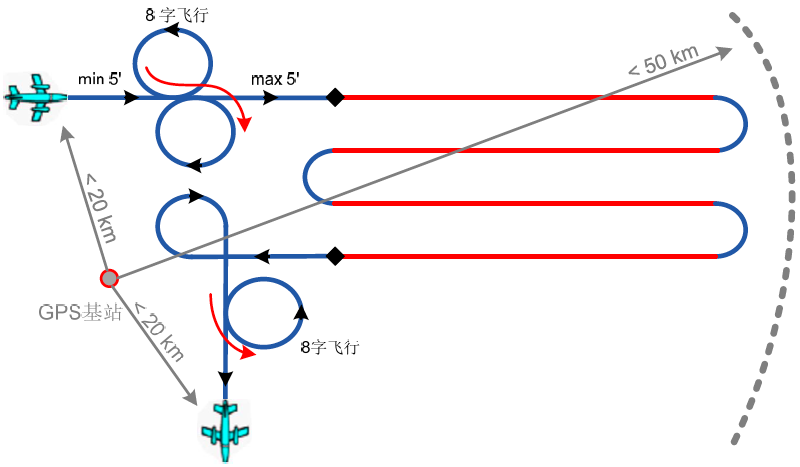
\includegraphics[width=0.7\linewidth]{figure/Chapter5/飞行质量要求}
			 \caption{飞行质量要求}
			 \label{fig:飞行质量要求}
		\end{figure}
	\item \textbf{飞行作业和设备空中操作}:空中操作是固定而且单一的,高级的激光
		雷达设备在使用操作上往往十分简单,用
		户只需进行触动几个按钮就可以完成整个
		航飞任务,其他所有工作都让计算机来监
		视完成。
	\item 激光扫描测量
	\item GPS/IMU定位定向测量
	\item 数码相机拍摄
	\item 空中异常情况及处理
\end{enumerate}

\subsection{数据整理阶段}
\paragraph{数据检查与质量控制}
\begin{enumerate}
	\item \textbf{数据整理归档}
	\item \textbf{日志文件}
	\item \textbf{数据质量检查}
		\begin{itemize}
			\item GPS/IMU数据解压
			\item 导航文件精度指标
			\item 激光数据检查
			\item 影像数据检查
		\end{itemize}
	\item \textbf{补飞和重飞}
\end{enumerate}

\paragraph{数据预处理}
\begin{enumerate}
	\item \textbf{目的}:
		\begin{itemize}
			\item 三维坐标解算
			\item 坐标转换
			\item 文件生成
		\end{itemize}
	\item \textbf{数据预处理流程}:如图\ref{fig:数据预处理流程}所示。
		\begin{figure}[htbp]
			\centering
			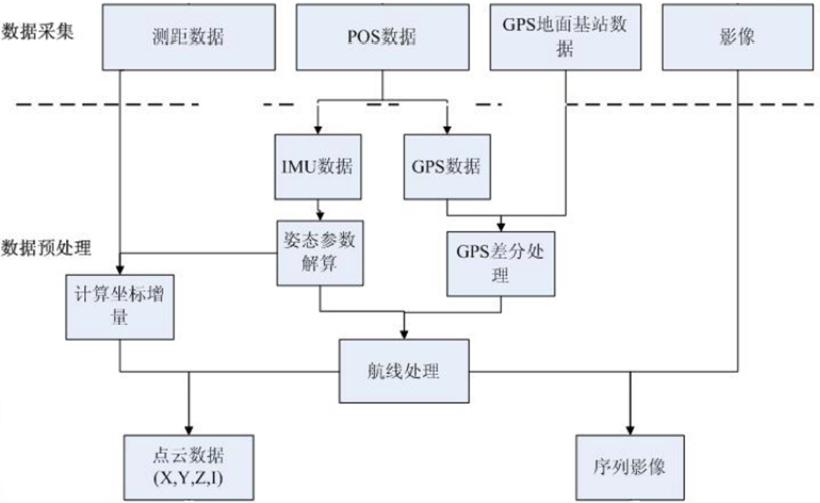
\includegraphics[width=0.5\linewidth]{figure/Chapter5/数据预处理流程}
			\caption{数据预处理流程}
			\label{fig:数据预处理流程}
		\end{figure}
	\item \textbf{SBET (Smoothed Best Estimated Trajectory)航迹文件处理}:GPS差分处理(GPS数据+基站数据)。每条航带一个航迹文件,处理软件 POSProc。
	\item \textbf{位置内插}。如图所示。
		\begin{figure}[htbp]
			\centering
			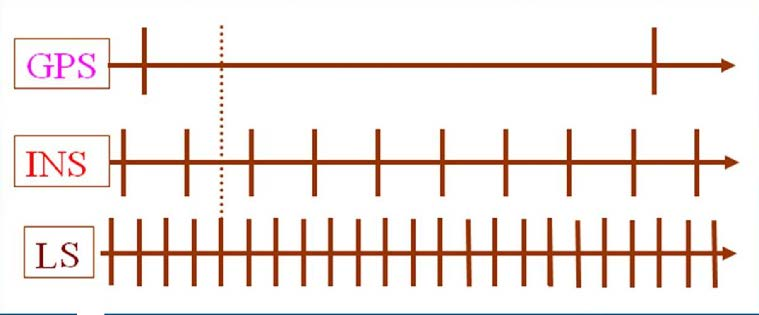
\includegraphics[width=0.5\linewidth]{figure/Chapter5/位置内插}
			\caption{位置内插}
			\label{fig:位置内插}
		\end{figure}
	\item \textbf{“*.LAS” 文件——ALS Post Processor}
		\begin{itemize}
			\item 解算每个目标点的三维坐标;
			\item 每条航带生成一个二进制格式的LAS文件;
			\item 存储格式为lat/lon/el/intensity data 或者 northing/easting/el/intensity in user-selected projection;
			\item 记录顺序:shot-by shot, return by return。
		\end{itemize}
	\item \textbf{生成 “quick-look edge-of-coverage” 高程图 ( *.TIF)}
\end{enumerate}

\paragraph{调整航带间点云不一致}如图\ref{fig:调整航带间点云不一致}所示。
\begin{figure}[htbp]
	\centering
	\subfloat[原始点云]{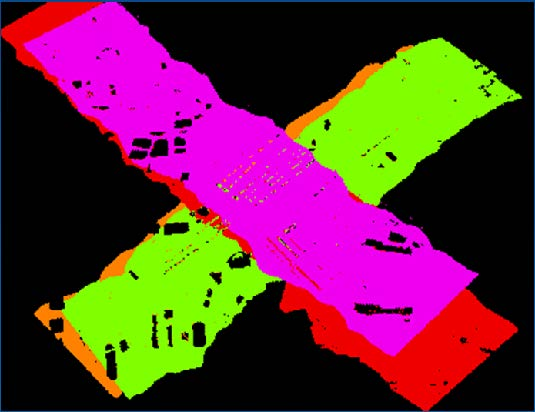
\includegraphics[height=2.5cm]{figure/Chapter5/原始点云}}
	\subfloat[调整前点云]{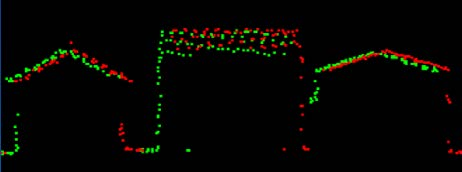
\includegraphics[height=2.5cm]{figure/Chapter5/调整前点云}}
	\subfloat[调整后点云]{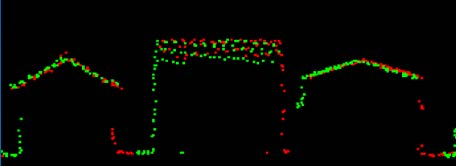
\includegraphics[height=2.5cm]{figure/Chapter5/调整后点云}}
	\caption{调整航带间点云不一致}
	\label{fig:调整航带间点云不一致}
\end{figure}

\paragraph{坐标变换}由WGS84坐标系大地坐标变换为地方局部坐标系坐标。
\begin{itemize}
	\item \textbf{投影变换}
		\begin{itemize}
			\item Gauss投影
			\item UTM投影
			\item Mercator投影
			\item Lambert投影
			\item Albers投影
		\end{itemize}
	\item \textbf{椭球变换}
		\begin{itemize}
			\item \textit{七参数法}(包括布尔莎模型、一步法模型、海尔曼特等),即$ X $平移,$ Y $平 移,$ Z $平移,$ X $旋转,$ Y $旋转,$ Z $旋转,尺度变化$ K $。
			\item \textit{三参数}(莫洛登斯基模型),即$ X $平移,$ Y $平移,$ Z $平移,而将$ X $旋转,$ Y $旋转,$ Z $旋转,尺度变化$ K $视为0,所以三参数只是七参数的一种特例。
		\end{itemize}
\end{itemize}

\paragraph{文件生成}
\begin{enumerate}
	\item \textbf{LAS格式}:美国摄影测量与遥感协会提出Lidar Data Exchange Format Standard (LDEFS) 1.0标准。
		\begin{itemize}
			\item \textbf{公共数据块(Public Header Block)}:公共数据块的大小是227 bytes,记录了关于该文件的一些基本信息,
				如:文件标识、飞行时间、回波个数、坐标范围等等,详细描述了关于las数据采集的信息。
			\item \textbf{变长数据记录(Variable length Records)}。
			\item \textbf{点数据块(Point data)}。
			\item \textbf{变长的波形记录}(1.3格式)。
		\end{itemize}
	\item \textbf{ASC栅格格式}:一些公司采用了栅格文件格式作为Lidar的数据格式。例如,采用ArcInfo Grid格式的数据作为通用格式。
		\begin{itemize}
			\item \textbf{头部信息}:
				\begin{itemize}
					\item ncols行数
					\item nrows列数
					\item xllcenter中心点x坐标
					\item yllcenter中心点y坐标
					\item cellsize采样间距
					\item NODATA\_value -9999.000000(无效数据)
				\end{itemize}
			\item \textbf{数据信息}:记录具体的信息数据。
		\end{itemize}
	\item \textbf{自定义TXT格式}:这种格式直接以文本的方式记录LiDAR数据,每 一行记录一束激光的回波数据,以不同的列记录不同属性的数据,一般会在数据中加以说明。
\end{enumerate}

\paragraph{点云数据特点}LiDAR激光脚点的分布是按照时间序列进行采样和存储的,其在地面上的分布不是规则的,其空间分布呈现为离散的数据”点云”(Points Cloud)。如图\ref{fig:点云数据特点}所示。
\begin{figure}[htbp]
	\centering
	\subfloat[激光脚点]{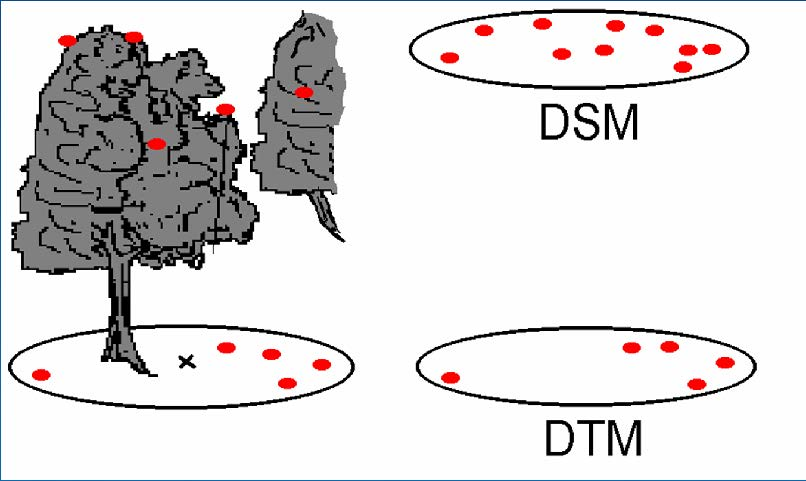
\includegraphics[height=4cm]{figure/Chapter5/点云数据特点_脚点}} \quad
	\subfloat[点云]{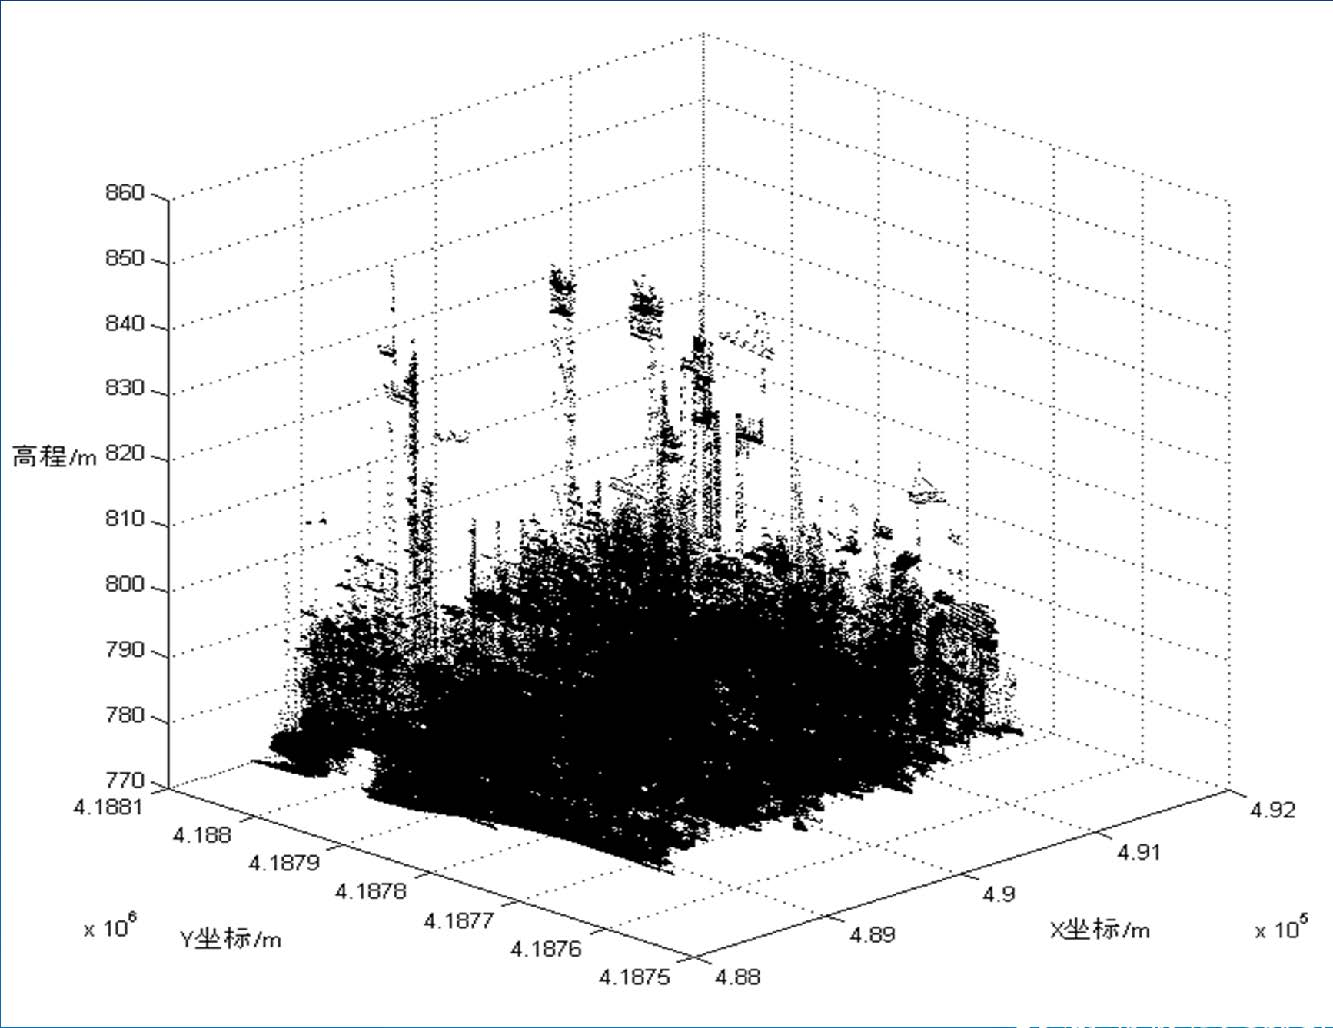
\includegraphics[height=4cm]{figure/Chapter5/点云数据特点_点云}}
	\caption{点云数据特点}
	\label{fig:点云数据特点}
\end{figure}

\section{LiDAR技术与同类技术对比}
\subsection{摄影测量与LiDAR的主要差异}
摄影测量与LiDAR的主要差异如表\ref{tab:摄影测量与LiDAR的主要差异}所示。

\LTXtable{\textwidth}{table/摄影测量与LiDAR的主要差异}

\subsection{LiDAR技术的优势}
\begin{enumerate}
	\item \textbf{对于极少纹理的地表面的测绘}
	\item \textbf{森林和植物覆盖物繁多的地域测绘}:茂密森林地区——机载LiDAR系统可以获得地形数据,而摄影测量系统做不到。
	\item \textbf{细长地物目标的测绘}:包括道路测绘、电力线及电线塔测绘、海岸侵蚀监测、水道水系测量、铁道线测绘、光纤通道量测、管道量测等。
		机载LiDAR系统的扫描带较窄,在上述各种地物量测方面的 效率成本比要高得多,对于相关的管理、规划、设计工作,都能提供有效的信息。
	\item \textbf{城市区域DSM的生成}:由于机载LiDAR系统可以进行密集的高精度量测,对于不连续、突出的三维目标,特别是建筑物的检测、重建,比人工量测速度快得多。
		可为城市规划、通讯天线的安置等工作,提供非常重要的数据。
	\item \textbf{需要高密度和高精度量测的区域}:\begin{itemize}
			\item 露天矿监测
			\item 露天堆集物监测
			\item 洪水测绘
			\item 局部超级设施(如飞机场)的测绘
		\end{itemize}
	\item \textbf{微小目标量测}:航摄影像中很难发现,人工测量无法进行的工作,如电力线量测等。
	\item \textbf{需要快速响应的应用领域}:如自然灾害监测,需要很快提供信息数据时,由于机载激光系统可以进行直接测距,转换为三维坐标,因此成为极其重要的工具。
\end{enumerate}

\subsection{LiDAR与INSAR的比较}
LiDAR与INSAR的比较如表\ref{tab:LiDAR与INSAR的比较}所示。

\LTXtable{\textwidth}{table/LiDAR与INSAR的比较}